\begin{exercise}
      {ID-9928ff2c0f0ec6d6703eed3f2995a158a99c91dc}
      {Rohre}
  \ifproblem\problem
    \begin{minipage}{0.2\textwidth}
      \centering
      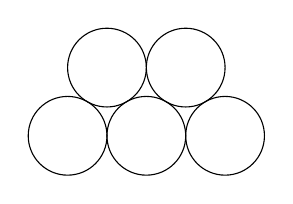
\begin{tikzpicture}
        % unten
        \draw (0, 0) circle (5mm);
        \draw (1, 0) circle (5mm);
        \draw (2, 0) circle (5mm);
        % oben
        \draw (0.5, 0.866) circle (5mm);
        \draw (1.5, 0.866) circle (5mm);
      \end{tikzpicture}%
    \end{minipage}\hfill
    \begin{minipage}{0.75\textwidth}
      Fünf Rohre mit einem Durchmesser von jeweils \simeter{1} werden auf einen Anhänger
      geladen -- drei Rohre in der unteren Reihe, zwei versetzt darüber.
      Wie hoch ist die Ladung?
    \end{minipage}
  \fi
  \ifoutline\outline
    \begingroup
      \dimen1=5cm%
      \begin{minipage}{\dimen1}
        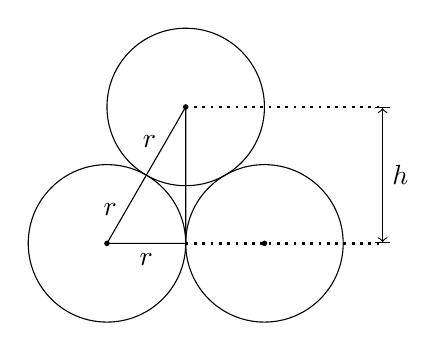
\begin{tikzpicture}
          % Rohre
          \draw (0, 0) circle[radius=1cm];
          \draw (2, 0) circle[radius=1cm];
          \draw (1, 1.7321) circle[radius=1cm];
          % Mittelpunkte
          \fill (0, 0) circle[radius=1pt];
          \fill (2, 0) circle[radius=1pt];
          \fill (1, 1.7321) circle[radius=1pt];
          % Dreieck
          \draw (0, 0)      -- node[below]{$r$}
                (1, 0)      --
                (1, 1.7321) -- node[left, pos=0.25]{$r$}
                               node[left, pos=0.75]{$r$}
                cycle;
          % Hoehe
          \draw[|<->|] (3.5, 0) -- node[right]{$h$}
                       (3.5, 1.7321);
          \draw[style=dotted, line width=1pt] (1, 0) -- (3.5, 0);
          \draw[style=dotted, line width=1pt] (1, 1.7321) -- (3.5, 1.7321);
        \end{tikzpicture}%
      \end{minipage}%
      \dimen2=\linewidth%
      \advance\dimen2 by -\dimen1%
      \begin{minipage}{\dimen2}
        \setlength{\abovedisplayskip}{0pt}%
        \begin{equation*}
          (2r)^2=r^2+h^2
        \end{equation*}
      \end{minipage}%
    \endgroup
  \fi
  \ifoutcome\outcome
    Die Ladung ist ca. \simeter{1.866} hoch.
  \fi
\end{exercise}
